\documentclass[11pt]{article}

\usepackage[margin=1in]{geometry}
\usepackage{fancyhdr}
\usepackage{amsmath,amsfonts,amsthm,bm}
\usepackage{amssymb}
\pagestyle{fancy}


\usepackage[T1]{fontenc}
\usepackage{CJKutf8}

\CJKencfamily{UTF8}{bkai} % 使用標楷體


\AtBeginDocument{%
    \begin{CJK}{UTF8}{bkai}} % 使用標楷體
    \AtEndDocument{%
    \clearpage\end{CJK}}
    
\usepackage{pgfplots} % for histogram plotting

\pgfplotsset{
  compat=newest,
  xlabel near ticks,
  ylabel near ticks
}
    
\usepackage{pgf,tikz}
\usepackage{mathrsfs}
\usetikzlibrary{arrows}
\usetikzlibrary[patterns]
\usetikzlibrary{positioning}
\newdimen\nodeDist
\nodeDist=28mm

\setlength{\unitlength}{1pt}

\pgfdeclarepatternformonly[\GridSize]{MyGrid}{\pgfqpoint{-1pt}{-1pt}}{\pgfqpoint{4pt}{4pt}}{\pgfqpoint{\GridSize}{\GridSize}}%
{
  \pgfsetlinewidth{0.3pt}
  \pgfpathmoveto{\pgfqpoint{0pt}{0pt}}
  \pgfpathlineto{\pgfqpoint{0pt}{3.1pt}}
  \pgfpathmoveto{\pgfqpoint{0pt}{0pt}}
  \pgfpathlineto{\pgfqpoint{3.1pt}{0pt}}
  \pgfusepath{stroke}
}

\pgfdeclarepatternformonly[\GridSize]{MyGrid2}{\pgfqpoint{-1pt}{-1pt}}{\pgfqpoint{4pt}{4pt}}{\pgfqpoint{\GridSize}{\GridSize}}%
{
  \pgfsetlinewidth{0.3pt}
  \pgfpathmoveto{\pgfqpoint{0pt}{0pt}}
  \pgfpathlineto{\pgfqpoint{0pt}{-30pt}}
  \pgfpathmoveto{\pgfqpoint{0pt}{0pt}}
  \pgfpathlineto{\pgfqpoint{-30pt}{0pt}}
  \pgfusepath{stroke}
}

\newdimen\GridSize
\tikzset{
    GridSize/.code={\GridSize=#1},
    GridSize=3pt
}



\definecolor{qqqqff}{rgb}{0.,0.,1.}
\definecolor{ffqqqq}{rgb}{1.,0.,0.}
\definecolor{qqwuqq}{rgb}{0.,0.39215686274509803,0.}
\definecolor{cqcqcq}{rgb}{0.7529411764705882,0.7529411764705882,0.7529411764705882}

\usepackage{enumitem}
\usepackage{fancybox}
\usepackage{sectsty}
\allsectionsfont{\centering}
\PassOptionsToPackage{hyphens}{url}\usepackage[colorlinks=true, urlcolor=black, hyperfootnotes=false]{hyperref}

\lhead{Machine Learning Techniques (NTU, Spring 2017)}
\chead{}
\rhead{王冠鈞(b03902027)}



\begin{document}


\section*{Homework \#3}
\subsection*{Answer Sheet}
\begin{center}
DEADLINE: 05/23/2017, 14:00\\
INSTRUCTOR:  Hsuan-Tien Lin\\[0.5cm]
王冠鈞 b03902027
\end{center}


\begin{enumerate}[label=\textbf{\arabic*}.]
	\item To let the weighted-$E_{\text{in}}$ optimization problem equivalent to a usual $E_{\text{in}}$ optimization problem, that is, \[(P_1)\ \underset{\mathbf{w}}\min\ E_{\text{in}}(\mathbf{w}) = \frac{1}{N} \sum_{n=1}^{N} (\tilde{y}_n - \mathbf{w}^T\tilde{\mathbf{x}}_n)^2\], we can observe the original problem, and we can find that it can be written as:\[(P_2)\ \underset{\mathbf{w}}\min\ E_{\text{in}}(\mathbf{w}) = \frac{1}{N} \sum_{n=1}^{N} ((\sqrt{u_n}y_n) - \mathbf{w}^T(\sqrt{u_n}\mathbf{x}_n))^2\] Apparently, the condition that $P_1\equiv P_2$ is:\[(\tilde{\mathbf{x}}_n, \tilde{y}_n)=(\sqrt{u_n}\mathbf{x}_n, \sqrt{u_n}y_n),\ \text{for }n=1, 2, \cdots, N\]

  \item In the first iteration, $u_+^{(1)}=u_-^{(1)}$, and $\epsilon_1 = \frac{\sum_{n=1}^N u_n^{(1)}[\![y_n \neq g_1(\mathbf{x}_n)]\!]}{\sum_{n=1}^{N} u_n^{(1)}} = \frac{0.01N\times u_-^{(1)}}{0.99N\times u_+^{(1)}+0.01N\times u_-^{(1)}}=0.01$. According to the algorithm, after updating the weights, we get:
  \begin{align*}
    u_+^{(2)} = u_+^{(1)}\div\sqrt{\frac{1-\epsilon_1}{\epsilon_1}} = u_+^{(1)}\sqrt{\frac{0.01}{0.99}}\\
    u_-^{(2)} = u_-^{(1)}\times\sqrt{\frac{1-\epsilon_1}{\epsilon_1}} = u_-^{(1)}\sqrt{\frac{0.99}{0.01}}
  \end{align*}
  And finally, we get \[\frac{u_+^{(2)}}{u_-^{(2)}} = \frac{u_+^{(1)}\sqrt{\frac{0.01}{0.99}}}{u_-^{(1)}\sqrt{\frac{0.99}{0.01}}} = \frac{u_+^{(1)}\times0.01}{u_-^{(1)}\times 0.99} = \frac{1}{99}\]

  \item First, regardless of the number of dimensions, there are universally 2 decision stumps that return 1/-1 , respectively, for every input. Then, for every dimension, all data points are on the integer point in interval $[L, R]$, and there are $R-L$ spaces in the interval, and every space can accommodate 2 "different" decision stumps (positive/negative rays) that will output $1$ for some inputs and $-1$ for others. Thus, in general, there are $2 + 2d \times (R - L)$ different decision stumps in total, and in this question ($d=2, L=1, R=6$), there are $2 + 2 \times 2 \times (6 - 1) = 22$ different stumps.

  \item First, since all $g_i(\mathbf{x})$ returns either $1$ or $-1$, and the kernel is equal to:
  \[K_{ds}(\mathbf{x}, \mathbf{x'})=(\bm{\phi}_{ds}(\mathbf{x}))^T (\bm{\phi}_{ds}(\mathbf{x'})) = \sum_{t=1}^{\mathcal{|G|}}g_t(\mathbf{x})g_t(\mathbf{x'})\]
  , which is a sum of 1-s and $-1$-s. The sign depends on whether $g_t(\mathbf{x})$ and $g_t(\mathbf{x'})$ are both positive/negative or not. We first notice that when $g(\mathbf{x}) = 1$ or $g(\mathbf{x}) = -1$, the products will definitely be positive, while in other cases it depends. We can consider the kernel function is equivalent to the following:\[\begin{aligned}K_{ds}(\mathbf{x}, \mathbf{x'})&= \text{ \# of all different decision stumps } - 2\times \text{ \# of decision stumps that will separate }\mathbf{x} \text{ and }\mathbf{x'} \\ & = |\mathcal{G}| - 2\times \text{ \# of decision stumps that will separate }\mathbf{x} \text{ and }\mathbf{x'} \end{aligned}\]
  The main concept is that we first assume that all $g_t(\mathbf{x})g_t(\mathbf{x'})$ are positive, giving us $|\mathcal{G}|$. However, the fact is that there may be some $t$ such that $g_t(\mathbf{x})g_t(\mathbf{x'}) = -1$, but since we previously added them as $1$, we have to subtract the number of negative terms by 2 times.\\
  Now we need to find the $\text{\# of decision stumps that will separate }\mathbf{x} \text{ and }\mathbf{x'}$. For convenience to explain, consider a 2-dimensional space with $R-L=6$:

  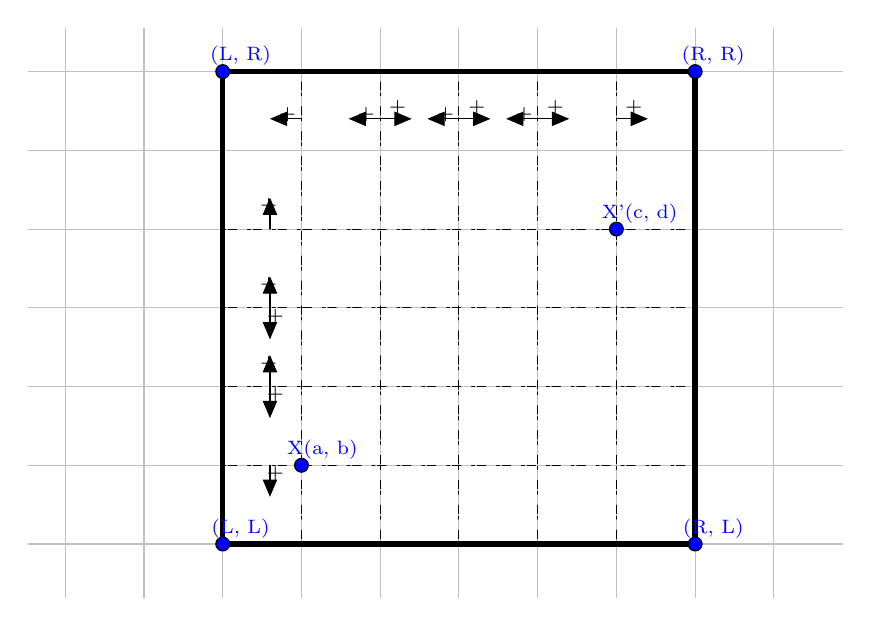
\begin{tikzpicture}[line cap=round,line join=round,>=triangle 45,x=1.0cm,y=1.0cm]
\draw [color=cqcqcq,, xstep=1.0cm,ystep=1.0cm] (1.5301459496643384,1.319583821302476) grid (11.867913276354292,8.550773352357524);
\clip(1.5301459496643384,1.319583821302476) rectangle (11.867913276354292,8.550773352357524);
\draw [line width=2.pt] (4.,2.)-- (10.,2.);
\draw [line width=2.pt] (10.,2.)-- (10.,8.);
\draw [line width=2.pt] (10.,8.)-- (4.,8.);
\draw [line width=2.pt] (4.,8.)-- (4.,2.);
\draw [dash pattern=on 1pt off 1pt on 3pt off 4pt] (4.,6.)-- (10.,6.);
\draw [dash pattern=on 1pt off 1pt on 3pt off 4pt] (4.,5.)-- (10.,5.);
\draw [dash pattern=on 1pt off 1pt on 3pt off 4pt] (4.,4.)-- (10.,4.);
\draw [dash pattern=on 1pt off 1pt on 3pt off 4pt] (4.,3.)-- (10.,3.);
\draw [->] (4.6,3.) -- (4.6,2.6);
\draw [->] (4.6,4.) -- (4.6,3.6);
\draw [->] (4.6,4.) -- (4.6,4.4);
\draw [->] (4.6,5.) -- (4.6,4.6);
\draw [->] (4.6,5.) -- (4.6,5.4);
\draw [->] (4.6,6.) -- (4.6,6.4);
\draw [dash pattern=on 1pt off 1pt on 3pt off 4pt] (5.,2.)-- (5.,8.);
\draw [dash pattern=on 1pt off 1pt on 3pt off 4pt] (6.,2.)-- (6.,8.);
\draw [dash pattern=on 1pt off 1pt on 3pt off 4pt] (7.,2.)-- (7.,8.);
\draw [dash pattern=on 1pt off 1pt on 3pt off 4pt] (8.,2.)-- (8.,8.);
\draw [dash pattern=on 1pt off 1pt on 3pt off 4pt] (9.,2.)-- (9.,8.);
\draw [->] (5.,7.4) -- (4.6,7.4);
\draw [->] (6.,7.4) -- (5.6,7.4);
\draw [->] (6.,7.4) -- (6.4,7.4);
\draw [->] (7.,7.4) -- (6.6,7.4);
\draw [->] (7.,7.4) -- (7.4,7.4);
\draw [->] (8.,7.4) -- (7.6,7.4);
\draw [->] (8.,7.4) -- (8.4,7.4);
\draw [->] (9.,7.4) -- (9.4,7.4);
\begin{scriptsize}
\draw [fill=qqqqff] (5.,3.) circle (2.5pt);
\draw[color=qqqqff] (5.266435460630454,3.192976174413254) node {X(a, b)};
\draw [fill=qqqqff] (9.,6.) circle (2.5pt);
\draw[color=qqqqff] (9.296590438751208,6.1946020174927074) node {X'(c, d)};
\draw [fill=qqqqff] (4.,2.) circle (2.5pt);
\draw[color=qqqqff] (4.227411130333698,2.19593262513861) node {(L, L)};
\draw [fill=qqqqff] (10.,2.) circle (2.5pt);
\draw[color=qqqqff] (10.230662816492735,2.19593262513861) node {(R, L)};
\draw [fill=qqqqff] (10.,8.) circle (2.5pt);
\draw[color=qqqqff] (10.230662816492735,8.199184311297518) node {(R, R)};
\draw [fill=qqqqff] (4.,8.) circle (2.5pt);
\draw[color=qqqqff] (4.227411130333698,8.199184311297518) node {(L, R)};
\draw[color=black] (4.668209331065655,2.899110707258622) node {+};
\draw[color=black] (4.668209331065655,3.896154256533266) node {+};
\draw[color=black] (4.584247769021473,4.294971676243123) node {+};
\draw[color=black] (4.668209331065655,4.893197805807909) node {+};
\draw[color=black] (4.584247769021473,5.292015225517767) node {+};
\draw[color=black] (4.584247769021473,6.299553970047933) node {+};
\draw[color=black] (4.825637259898497,7.454025448155416) node {+};
\draw[color=black] (5.822680809173162,7.454025448155416) node {+};
\draw[color=black] (6.2214982288830285,7.537987010199596) node {+};
\draw[color=black] (6.830219553703351,7.454025448155416) node {+};
\draw[color=black] (7.229036973413217,7.537987010199596) node {+};
\draw[color=black] (7.827263102978017,7.454025448155416) node {+};
\draw[color=black] (8.226080522687882,7.537987010199596) node {+};
\draw[color=black] (9.223124071962548,7.537987010199596) node {+};
\end{scriptsize}
\end{tikzpicture}

In this figure, it has explicitly illustrated that the decision stumps that will separate the two points (the dot-dash lines segments) are within the intervals $[a, c]$ in the 1st dimension and $[b, d]$ in the 2nd dimension.\footnote{The arrows denotes the positive direction of a decision stump.} Thus the number of such decision stumps in this example is $2\times((c-a)+(d-b))=2d_1(\mathbf{x}, \mathbf{x'})$, where $d_1(\mathbf{x}, \mathbf{x'})$ is the $L_1$ distance\footnote{Also called the \textit{taxicab distance}, \textit{$l_1$ norm} or the \textit{Manhattan distance}. See the following reference: \url{https://en.wikipedia.org/wiki/Taxicab_geometry}.} of the two vectors. This can be expanded to any finite dimensions without modification. Finally, the overall formula of the kernel can be written as:
\[\begin{aligned} K_{ds}(\mathbf{x}, \mathbf{x'}) &= |\mathcal{G}|-2\times 2d_1(\mathbf{x}, \mathbf{x'}) \\ &= 2 + 2d \times (R - L) - 4d_1(\mathbf{x}, \mathbf{x'}) \end{aligned} \]
In the case of the previous problem, $K_{ds}(\mathbf{x}, \mathbf{x'}) = 22 - 4d_1(\mathbf{x}, \mathbf{x'})$.\\
As for the "bonus" part for non-integers, without any other conditions I don't think that there's a solution since the number of decision stumps will become infinite, and it's meaningless to compare the difference between the infinite number of decision stumps and the infinite number of the decision stumps that will separate the two input vectors. (Unless we still use the "finite" decision stumps with the "integer" constraint, and the answer will be $2d \times (R - L) - 4d_1(\lfloor\mathbf{x}\rfloor, \lfloor\mathbf{x'}\rfloor)$, where $\lfloor\mathbf{x}\rfloor$ is the floor operation of each term in $\mathbf{x}$.)

  \item We can simply get $1-\mu_+^2-\mu_-^2=1-\mu_+^2-(1-\mu_+)^2=2(\mu_+-\mu_+^2)$. We can find its minimum by differentiating:
  \[\begin{aligned}
  &\frac{d}{d\mu_+}2(\mu_+-\mu_+^2) = 2-4\mu_+=0\Rightarrow \mu_+ = \frac{1}{2}\\
  \Rightarrow\mkern40mu &\min(1-\mu_+^2-\mu_-^2) = 1-(\frac{1}{2})^2-(1-\frac{1}{2})^2=\frac{1}{2}
  \end{aligned}\]

  \item I'll justify the errors below that whether they can be written in the form $k(\mu_+-\mu_+^2)$:
  \begin{enumerate}[label={[\textbf{\alph*}]}]
    \item $\min(\mu_+, \mu_-) = \min(\mu_+, 1-\mu_+)$, cannot be simplified to $k(\mu_+-\mu_+^2)$.
    \item $\begin{aligned} \mu_+(1-(\mu_+ - \mu_-))^2+ \mu_-(-1-(\mu_+ - \mu_-))^2 & = \mu_+(1-\mu_+ + \mu_-)^2+ \mu_-(-1-\mu_+ + \mu_-)^2\\& = \mu_+(2\mu_-)^2+\mu_-(-2\mu_+)^2\\ & = 4(\mu_+\mu_-^2 + \mu_+^2\mu_-)\\ & = 4(\mu_+(1-\mu_+)^2+\mu_+^2(1-\mu_+))\\& = 4(\mu_+-2\mu_+^2+\mu_+^3+\mu_+^2-\mu_+^3) \\ & = 4(\mu_+- \mu_+^2) \\ & = 2\times \text{Gini index} \end{aligned}$
    \item Apparently the logarithm cannot be simplified to some form of quadratic polynomial.
    \item $\begin{aligned} 1 - |\mu_+-\mu_-| = 1 - |\mu_+-1+ \mu_+| = 1 - |2\mu_+-1|\end{aligned}$, unlikely to further simplify to $k(\mu_+-\mu_+^2)$.
  \end{enumerate}
  From above, we conclude that the answer is [\textbf{b}] (the squared regression error).

  \item The relation between $t$ and $E_\text{in}(g_t)$ is shown below.\footnote{All plots is this answer sheet are made with GNU Octave.} According to the results, $E_\text{in}(g_1)=0.24, \alpha_1 = 0.573640$.\\
\begin{picture}(0,0)
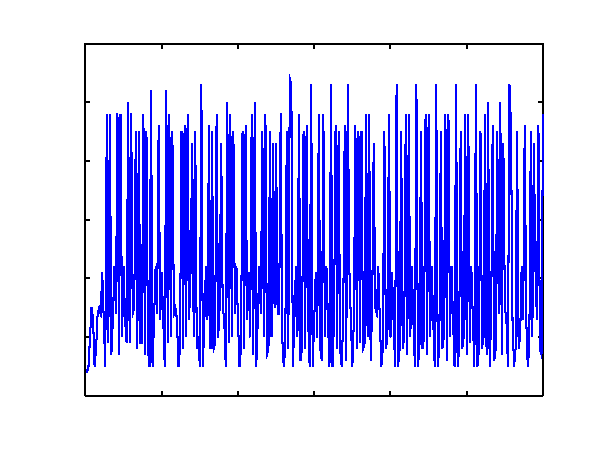
\includegraphics{plots/q7-inc}
\end{picture}%
\begin{picture}(288,218)(0,0)
\fontsize{10}{0}
\selectfont\put(41.0044,22.9956){\makebox(0,0)[t]{\textcolor[rgb]{0,0,0}{{0}}}}
\fontsize{10}{0}
\selectfont\put(77.6104,22.9956){\makebox(0,0)[t]{\textcolor[rgb]{0,0,0}{{50}}}}
\fontsize{10}{0}
\selectfont\put(114.216,22.9956){\makebox(0,0)[t]{\textcolor[rgb]{0,0,0}{{100}}}}
\fontsize{10}{0}
\selectfont\put(150.822,22.9956){\makebox(0,0)[t]{\textcolor[rgb]{0,0,0}{{150}}}}
\fontsize{10}{0}
\selectfont\put(187.428,22.9956){\makebox(0,0)[t]{\textcolor[rgb]{0,0,0}{{200}}}}
\fontsize{10}{0}
\selectfont\put(224.034,22.9956){\makebox(0,0)[t]{\textcolor[rgb]{0,0,0}{{250}}}}
\fontsize{10}{0}
\selectfont\put(260.64,22.9956){\makebox(0,0)[t]{\textcolor[rgb]{0,0,0}{{300}}}}
\fontsize{10}{0}
\selectfont\put(36.0127,27.9961){\makebox(0,0)[r]{\textcolor[rgb]{0,0,0}{{0.2}}}}
\fontsize{10}{0}
\selectfont\put(36.0127,56.1631){\makebox(0,0)[r]{\textcolor[rgb]{0,0,0}{{0.3}}}}
\fontsize{10}{0}
\selectfont\put(36.0127,84.3306){\makebox(0,0)[r]{\textcolor[rgb]{0,0,0}{{0.4}}}}
\fontsize{10}{0}
\selectfont\put(36.0127,112.498){\makebox(0,0)[r]{\textcolor[rgb]{0,0,0}{{0.5}}}}
\fontsize{10}{0}
\selectfont\put(36.0127,140.666){\makebox(0,0)[r]{\textcolor[rgb]{0,0,0}{{0.6}}}}
\fontsize{10}{0}
\selectfont\put(36.0127,168.833){\makebox(0,0)[r]{\textcolor[rgb]{0,0,0}{{0.7}}}}
\fontsize{10}{0}
\selectfont\put(36.0127,197){\makebox(0,0)[r]{\textcolor[rgb]{0,0,0}{{0.8}}}}
\fontsize{10}{0}
\selectfont\put(150.822,11.9956){\makebox(0,0)[t]{\textcolor[rgb]{0,0,0}{{t}}}}
\fontsize{10}{0}
\selectfont\put(17.0127,112.498){\rotatebox{90}{\makebox(0,0)[b]{\textcolor[rgb]{0,0,0}{{$E_{in}(g_t)$}}}}}
\fontsize{10}{0}
\selectfont\put(150.822,207){\makebox(0,0)[b]{\textcolor[rgb]{0,0,0}{{Result of Question 7}}}}
\end{picture}

  \item Obviously, $E_\text{in}(g_t)$ is neither increasing or decreasing. It fluctuates between roughly 0.3 and 0.7, and it seems to have cycles up and down. A Possibility is that after a hypothesis is chosen, the wrong data will be emphasized with larger weight and may more likely to be correctly classified in the nest iteration, but the in-sample errors may have a large difference (since the weights are adjusted to make the previous one have the worst performance in terms of weighted in-sample error), which makes the $E_\text{in}(g_{t+1})$ when $E_\text{in}(g_t)$ is low and $E_\text{in}(g_{t+1})$ decrease when $E_\text{in}(g_t)$ is high.


  \item The relation between $t$ and $E_\text{in}(G_t)$ is shown below. According to the results, $E_\text{in}(G)=0$.\\
  \begin{picture}(0,0)
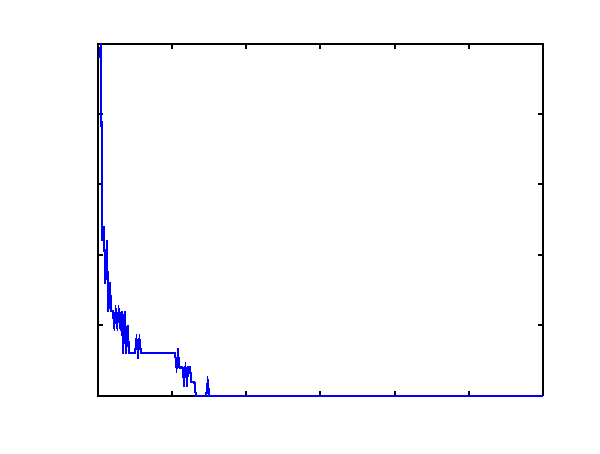
\includegraphics{plots/q9-inc}
\end{picture}%
\begin{picture}(288,218)(0,0)
\fontsize{10}{0}
\selectfont\put(47.0044,22.9956){\makebox(0,0)[t]{\textcolor[rgb]{0,0,0}{{0}}}}
\fontsize{10}{0}
\selectfont\put(82.6104,22.9956){\makebox(0,0)[t]{\textcolor[rgb]{0,0,0}{{50}}}}
\fontsize{10}{0}
\selectfont\put(118.216,22.9956){\makebox(0,0)[t]{\textcolor[rgb]{0,0,0}{{100}}}}
\fontsize{10}{0}
\selectfont\put(153.822,22.9956){\makebox(0,0)[t]{\textcolor[rgb]{0,0,0}{{150}}}}
\fontsize{10}{0}
\selectfont\put(189.428,22.9956){\makebox(0,0)[t]{\textcolor[rgb]{0,0,0}{{200}}}}
\fontsize{10}{0}
\selectfont\put(225.034,22.9956){\makebox(0,0)[t]{\textcolor[rgb]{0,0,0}{{250}}}}
\fontsize{10}{0}
\selectfont\put(260.64,22.9956){\makebox(0,0)[t]{\textcolor[rgb]{0,0,0}{{300}}}}
\fontsize{10}{0}
\selectfont\put(42.0132,27.9961){\makebox(0,0)[r]{\textcolor[rgb]{0,0,0}{{0}}}}
\fontsize{10}{0}
\selectfont\put(42.0132,61.7969){\makebox(0,0)[r]{\textcolor[rgb]{0,0,0}{{0.05}}}}
\fontsize{10}{0}
\selectfont\put(42.0132,95.5977){\makebox(0,0)[r]{\textcolor[rgb]{0,0,0}{{0.1}}}}
\fontsize{10}{0}
\selectfont\put(42.0132,129.398){\makebox(0,0)[r]{\textcolor[rgb]{0,0,0}{{0.15}}}}
\fontsize{10}{0}
\selectfont\put(42.0132,163.199){\makebox(0,0)[r]{\textcolor[rgb]{0,0,0}{{0.2}}}}
\fontsize{10}{0}
\selectfont\put(42.0132,197){\makebox(0,0)[r]{\textcolor[rgb]{0,0,0}{{0.25}}}}
\fontsize{10}{0}
\selectfont\put(153.822,11.9956){\makebox(0,0)[t]{\textcolor[rgb]{0,0,0}{{t}}}}
\fontsize{10}{0}
\selectfont\put(17.0132,112.498){\rotatebox{90}{\makebox(0,0)[b]{\textcolor[rgb]{0,0,0}{{$E_{in}(G_t)$}}}}}
\fontsize{10}{0}
\selectfont\put(153.822,207){\makebox(0,0)[b]{\textcolor[rgb]{0,0,0}{{Result of Question 9}}}}
\end{picture}

  \item The relation between $t$ and $U_t$ is shown below. According to the results, $U_2=0.854166, U_T=0.005465$.\\

  \begin{picture}(0,0)
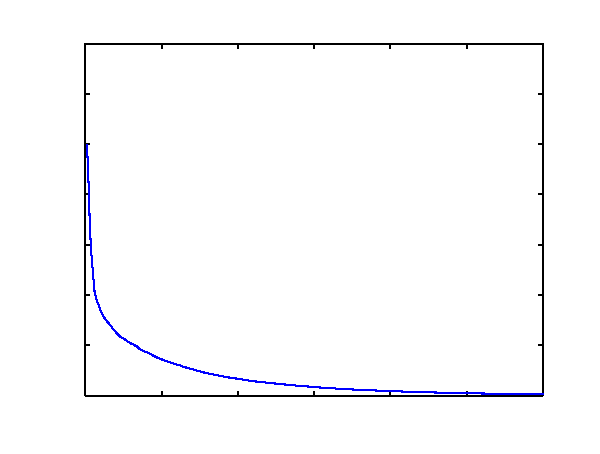
\includegraphics{plots/q10-inc}
\end{picture}%
\begin{picture}(288,218)(0,0)
\fontsize{10}{0}
\selectfont\put(41.0044,22.9956){\makebox(0,0)[t]{\textcolor[rgb]{0,0,0}{{0}}}}
\fontsize{10}{0}
\selectfont\put(77.6104,22.9956){\makebox(0,0)[t]{\textcolor[rgb]{0,0,0}{{50}}}}
\fontsize{10}{0}
\selectfont\put(114.216,22.9956){\makebox(0,0)[t]{\textcolor[rgb]{0,0,0}{{100}}}}
\fontsize{10}{0}
\selectfont\put(150.822,22.9956){\makebox(0,0)[t]{\textcolor[rgb]{0,0,0}{{150}}}}
\fontsize{10}{0}
\selectfont\put(187.428,22.9956){\makebox(0,0)[t]{\textcolor[rgb]{0,0,0}{{200}}}}
\fontsize{10}{0}
\selectfont\put(224.034,22.9956){\makebox(0,0)[t]{\textcolor[rgb]{0,0,0}{{250}}}}
\fontsize{10}{0}
\selectfont\put(260.64,22.9956){\makebox(0,0)[t]{\textcolor[rgb]{0,0,0}{{300}}}}
\fontsize{10}{0}
\selectfont\put(36.0127,27.9961){\makebox(0,0)[r]{\textcolor[rgb]{0,0,0}{{0}}}}
\fontsize{10}{0}
\selectfont\put(36.0127,52.1392){\makebox(0,0)[r]{\textcolor[rgb]{0,0,0}{{0.2}}}}
\fontsize{10}{0}
\selectfont\put(36.0127,76.2827){\makebox(0,0)[r]{\textcolor[rgb]{0,0,0}{{0.4}}}}
\fontsize{10}{0}
\selectfont\put(36.0127,100.426){\makebox(0,0)[r]{\textcolor[rgb]{0,0,0}{{0.6}}}}
\fontsize{10}{0}
\selectfont\put(36.0127,124.57){\makebox(0,0)[r]{\textcolor[rgb]{0,0,0}{{0.8}}}}
\fontsize{10}{0}
\selectfont\put(36.0127,148.713){\makebox(0,0)[r]{\textcolor[rgb]{0,0,0}{{1}}}}
\fontsize{10}{0}
\selectfont\put(36.0127,172.856){\makebox(0,0)[r]{\textcolor[rgb]{0,0,0}{{1.2}}}}
\fontsize{10}{0}
\selectfont\put(36.0127,197){\makebox(0,0)[r]{\textcolor[rgb]{0,0,0}{{1.4}}}}
\fontsize{10}{0}
\selectfont\put(150.822,11.9956){\makebox(0,0)[t]{\textcolor[rgb]{0,0,0}{{t}}}}
\fontsize{10}{0}
\selectfont\put(17.0127,112.498){\rotatebox{90}{\makebox(0,0)[b]{\textcolor[rgb]{0,0,0}{{$U_t$}}}}}
\fontsize{10}{0}
\selectfont\put(150.822,207){\makebox(0,0)[b]{\textcolor[rgb]{0,0,0}{{Result of Question 10}}}}
\end{picture}

  \item The relation between $t$ and $\epsilon_t$ is shown below. According to the results, $\min (\epsilon_t) = 0.178728$.\\

\begin{picture}(0,0)
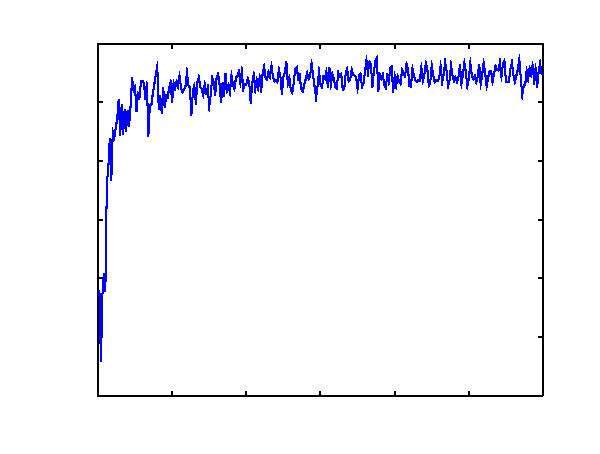
\includegraphics{plots/q11-inc}
\end{picture}%
\begin{picture}(288,218)(0,0)
\fontsize{10}{0}
\selectfont\put(47.0044,22.9956){\makebox(0,0)[t]{\textcolor[rgb]{0,0,0}{{0}}}}
\fontsize{10}{0}
\selectfont\put(82.6104,22.9956){\makebox(0,0)[t]{\textcolor[rgb]{0,0,0}{{50}}}}
\fontsize{10}{0}
\selectfont\put(118.216,22.9956){\makebox(0,0)[t]{\textcolor[rgb]{0,0,0}{{100}}}}
\fontsize{10}{0}
\selectfont\put(153.822,22.9956){\makebox(0,0)[t]{\textcolor[rgb]{0,0,0}{{150}}}}
\fontsize{10}{0}
\selectfont\put(189.428,22.9956){\makebox(0,0)[t]{\textcolor[rgb]{0,0,0}{{200}}}}
\fontsize{10}{0}
\selectfont\put(225.034,22.9956){\makebox(0,0)[t]{\textcolor[rgb]{0,0,0}{{250}}}}
\fontsize{10}{0}
\selectfont\put(260.64,22.9956){\makebox(0,0)[t]{\textcolor[rgb]{0,0,0}{{300}}}}
\fontsize{10}{0}
\selectfont\put(42.0132,27.9961){\makebox(0,0)[r]{\textcolor[rgb]{0,0,0}{{0.15}}}}
\fontsize{10}{0}
\selectfont\put(42.0132,56.1631){\makebox(0,0)[r]{\textcolor[rgb]{0,0,0}{{0.2}}}}
\fontsize{10}{0}
\selectfont\put(42.0132,84.3306){\makebox(0,0)[r]{\textcolor[rgb]{0,0,0}{{0.25}}}}
\fontsize{10}{0}
\selectfont\put(42.0132,112.498){\makebox(0,0)[r]{\textcolor[rgb]{0,0,0}{{0.3}}}}
\fontsize{10}{0}
\selectfont\put(42.0132,140.666){\makebox(0,0)[r]{\textcolor[rgb]{0,0,0}{{0.35}}}}
\fontsize{10}{0}
\selectfont\put(42.0132,168.833){\makebox(0,0)[r]{\textcolor[rgb]{0,0,0}{{0.4}}}}
\fontsize{10}{0}
\selectfont\put(42.0132,197){\makebox(0,0)[r]{\textcolor[rgb]{0,0,0}{{0.45}}}}
\fontsize{10}{0}
\selectfont\put(153.822,11.9956){\makebox(0,0)[t]{\textcolor[rgb]{0,0,0}{{t}}}}
\fontsize{10}{0}
\selectfont\put(17.0132,112.498){\rotatebox{90}{\makebox(0,0)[b]{\textcolor[rgb]{0,0,0}{{$\epsilon_t$}}}}}
\fontsize{10}{0}
\selectfont\put(153.822,207){\makebox(0,0)[b]{\textcolor[rgb]{0,0,0}{{Result of Question 11}}}}
\end{picture}

  \item The relation between $t$ and $E_\text{out}(g_t)$ is shown below. According to the results, $_\text{out}(g_1) = 0.29$.\\

\begin{picture}(0,0)
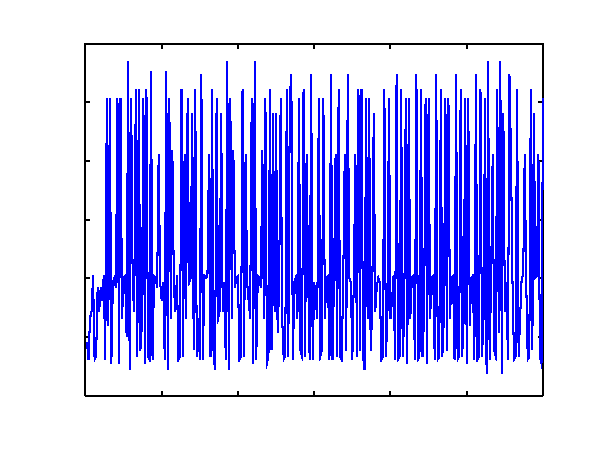
\includegraphics{plots/q12-inc}
\end{picture}%
\begin{picture}(288,218)(0,0)
\fontsize{10}{0}
\selectfont\put(41.0044,22.9956){\makebox(0,0)[t]{\textcolor[rgb]{0,0,0}{{0}}}}
\fontsize{10}{0}
\selectfont\put(77.6104,22.9956){\makebox(0,0)[t]{\textcolor[rgb]{0,0,0}{{50}}}}
\fontsize{10}{0}
\selectfont\put(114.216,22.9956){\makebox(0,0)[t]{\textcolor[rgb]{0,0,0}{{100}}}}
\fontsize{10}{0}
\selectfont\put(150.822,22.9956){\makebox(0,0)[t]{\textcolor[rgb]{0,0,0}{{150}}}}
\fontsize{10}{0}
\selectfont\put(187.428,22.9956){\makebox(0,0)[t]{\textcolor[rgb]{0,0,0}{{200}}}}
\fontsize{10}{0}
\selectfont\put(224.034,22.9956){\makebox(0,0)[t]{\textcolor[rgb]{0,0,0}{{250}}}}
\fontsize{10}{0}
\selectfont\put(260.64,22.9956){\makebox(0,0)[t]{\textcolor[rgb]{0,0,0}{{300}}}}
\fontsize{10}{0}
\selectfont\put(36.0127,27.9961){\makebox(0,0)[r]{\textcolor[rgb]{0,0,0}{{0.2}}}}
\fontsize{10}{0}
\selectfont\put(36.0127,56.1631){\makebox(0,0)[r]{\textcolor[rgb]{0,0,0}{{0.3}}}}
\fontsize{10}{0}
\selectfont\put(36.0127,84.3306){\makebox(0,0)[r]{\textcolor[rgb]{0,0,0}{{0.4}}}}
\fontsize{10}{0}
\selectfont\put(36.0127,112.498){\makebox(0,0)[r]{\textcolor[rgb]{0,0,0}{{0.5}}}}
\fontsize{10}{0}
\selectfont\put(36.0127,140.666){\makebox(0,0)[r]{\textcolor[rgb]{0,0,0}{{0.6}}}}
\fontsize{10}{0}
\selectfont\put(36.0127,168.833){\makebox(0,0)[r]{\textcolor[rgb]{0,0,0}{{0.7}}}}
\fontsize{10}{0}
\selectfont\put(36.0127,197){\makebox(0,0)[r]{\textcolor[rgb]{0,0,0}{{0.8}}}}
\fontsize{10}{0}
\selectfont\put(150.822,11.9956){\makebox(0,0)[t]{\textcolor[rgb]{0,0,0}{{t}}}}
\fontsize{10}{0}
\selectfont\put(17.0127,112.498){\rotatebox{90}{\makebox(0,0)[b]{\textcolor[rgb]{0,0,0}{{$E_{out}(g_t)$}}}}}
\fontsize{10}{0}
\selectfont\put(150.822,207){\makebox(0,0)[b]{\textcolor[rgb]{0,0,0}{{Result of Question 12}}}}
\end{picture}

  \item The relation between $t$ and $E_\text{out}(G_t)$ is shown below. According to the results, $_\text{out}(G) = 0.132$.\\

\begin{picture}(0,0)
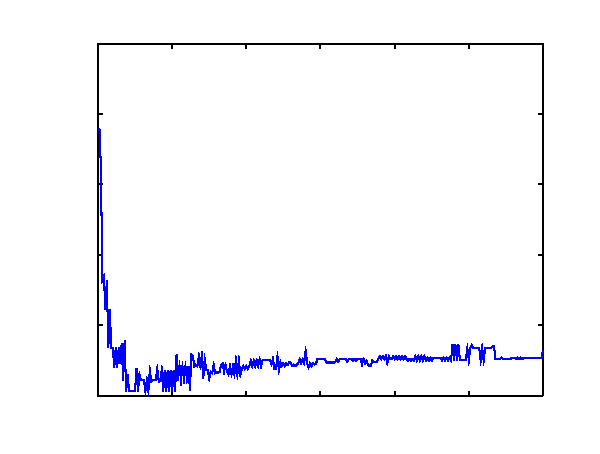
\includegraphics{plots/q13-inc}
\end{picture}%
\begin{picture}(288,218)(0,0)
\fontsize{10}{0}
\selectfont\put(47.0044,22.9956){\makebox(0,0)[t]{\textcolor[rgb]{0,0,0}{{0}}}}
\fontsize{10}{0}
\selectfont\put(82.6104,22.9956){\makebox(0,0)[t]{\textcolor[rgb]{0,0,0}{{50}}}}
\fontsize{10}{0}
\selectfont\put(118.216,22.9956){\makebox(0,0)[t]{\textcolor[rgb]{0,0,0}{{100}}}}
\fontsize{10}{0}
\selectfont\put(153.822,22.9956){\makebox(0,0)[t]{\textcolor[rgb]{0,0,0}{{150}}}}
\fontsize{10}{0}
\selectfont\put(189.428,22.9956){\makebox(0,0)[t]{\textcolor[rgb]{0,0,0}{{200}}}}
\fontsize{10}{0}
\selectfont\put(225.034,22.9956){\makebox(0,0)[t]{\textcolor[rgb]{0,0,0}{{250}}}}
\fontsize{10}{0}
\selectfont\put(260.64,22.9956){\makebox(0,0)[t]{\textcolor[rgb]{0,0,0}{{300}}}}
\fontsize{10}{0}
\selectfont\put(42.0132,27.9961){\makebox(0,0)[r]{\textcolor[rgb]{0,0,0}{{0.1}}}}
\fontsize{10}{0}
\selectfont\put(42.0132,61.7969){\makebox(0,0)[r]{\textcolor[rgb]{0,0,0}{{0.15}}}}
\fontsize{10}{0}
\selectfont\put(42.0132,95.5977){\makebox(0,0)[r]{\textcolor[rgb]{0,0,0}{{0.2}}}}
\fontsize{10}{0}
\selectfont\put(42.0132,129.398){\makebox(0,0)[r]{\textcolor[rgb]{0,0,0}{{0.25}}}}
\fontsize{10}{0}
\selectfont\put(42.0132,163.199){\makebox(0,0)[r]{\textcolor[rgb]{0,0,0}{{0.3}}}}
\fontsize{10}{0}
\selectfont\put(42.0132,197){\makebox(0,0)[r]{\textcolor[rgb]{0,0,0}{{0.35}}}}
\fontsize{10}{0}
\selectfont\put(153.822,11.9956){\makebox(0,0)[t]{\textcolor[rgb]{0,0,0}{{t}}}}
\fontsize{10}{0}
\selectfont\put(17.0132,112.498){\rotatebox{90}{\makebox(0,0)[b]{\textcolor[rgb]{0,0,0}{{$E_{out}(G_t)$}}}}}
\fontsize{10}{0}
\selectfont\put(153.822,207){\makebox(0,0)[b]{\textcolor[rgb]{0,0,0}{{Result of Question 13}}}}
\end{picture}

  \item Here is the tree drawn with \texttt{tikz}. Each leaf is tagged with a unique number, which will be used in question 16. Moreover, \texttt{x[0]} means the 0th feature of input data \texttt{x}.\\

  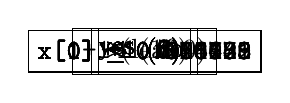
\begin{tikzpicture}[
    node/.style={%
      draw,
      rectangle,
    },
  ]

    \node [node] (A) {\texttt{x[1]} $\leq$ \texttt{0.626233}};
    \path (A) ++(-135:\nodeDist) node [node] (B) {\texttt{x[0]} $\leq$ \texttt{0.224440}};
    \path (B) ++(-135:\nodeDist) node [node] (D) {\texttt{x[1]} $\leq$ \texttt{0.115153}};
    \path (D) ++(-135:\nodeDist) node [node] (0) {\texttt{+1} (leaf 0)};
    \path (D) ++(-90:\nodeDist) node [node] (1) {\texttt{-1} (1)};
    \path (B) ++(-45:\nodeDist) node [node] (E) {\texttt{x[0]} $\geq$ \texttt{0.541508}};
    \path (E) ++(-135:\nodeDist) node [node] (F) {\texttt{x[1]} $\leq$ \texttt{0.285925}};
    \path (F) ++(-135:\nodeDist) node [node] (H) {\texttt{x[1]} $\leq$ \texttt{0.266039}};
    \path (H) ++(-135:\nodeDist) node [node] (2) {\texttt{+1} (2)};
    \path (H) ++(-90:\nodeDist) node [node] (3) {\texttt{-1} (3)};
    \path (F) ++(-90:\nodeDist) node [node] (4) {\texttt{+1} (4)};
    \path (E) ++(-45:\nodeDist) node [node] (G) {\texttt{x[1]} $\geq$ \texttt{0.358621}};
    \path (G) ++(-135:\nodeDist) node [node] (I) {\texttt{x[0]} $\leq$ \texttt{0.260752}};
    \path (I) ++(-135:\nodeDist) node [node] (5) {\texttt{+1} (5)};
    \path (I) ++(-90:\nodeDist) node [node] (6) {\texttt{-1} (6)};
    \path (G) ++(-45:\nodeDist) node [node] (J) {\texttt{x[0]} $\leq$ \texttt{0.501625}};
    \path (J) ++(-90:\nodeDist) node [node] (7) {\texttt{+1} (7)};
    \path (J) ++(-45:\nodeDist) node [node] (8) {\texttt{-1} (8)};

    \path (A) ++(-45:\nodeDist) node [node] (C) {\texttt{x[0]} $\leq$ \texttt{0.878171}};
    \path (C) ++(-90:\nodeDist) node [node] (9) {\texttt{-1} (9)};
    \path (C) ++(-45:\nodeDist) node [node] (10) {\texttt{+1} (10)};

    \draw (A) -- (B) node [left,pos=0.25] {yes}(A);
    \draw (B) -- (D) node [left,pos=0.25] {yes}(A);
    \draw (D) -- (0) node [left,pos=0.25] {yes}(A);
    \draw (D) -- (1) node [right,pos=0.25] {no}(A);
    \draw (B) -- (E) node [right,pos=0.25] {no}(A);
    \draw (E) -- (F) node [left,pos=0.25] {yes}(A);
    \draw (F) -- (H) node [left,pos=0.25] {yes}(A);
    \draw (H) -- (2) node [left,pos=0.25] {yes}(A);
    \draw (H) -- (3) node [right,pos=0.25] {no}(A);
    \draw (F) -- (4) node [right,pos=0.25] {no}(A);
    \draw (E) -- (G) node [right,pos=0.25] {no}(A);
    \draw (G) -- (I) node [left,pos=0.25] {yes}(A);
    \draw (I) -- (5) node [left,pos=0.25] {yes}(A);
    \draw (I) -- (6) node [right,pos=0.25] {no}(A);
    \draw (G) -- (J) node [right,pos=0.25] {no}(A);
    \draw (J) -- (7) node [left,pos=0.25] {yes}(A);
    \draw (J) -- (8) node [right,pos=0.25] {no}(A);

    \draw (A) -- (C) node [right,pos=0.25] {no}(A);
    \draw (C) -- (9) node [left,pos=0.25] {yes}(A);
    \draw (C) -- (10) node [right,pos=0.25] {no}(A);
\end{tikzpicture}

  \item According to the result, $E_{\text{in}} = 0$ and $E_{\text{out}} = 0.126$.

  \item According to the result, the lowest $E_{\text{in}}$ achievable by pruning a leaf is $0.01$ (pruning leaf 0, 3, 5 or 8, where the leaf numbers are listed in question 14), and the lowest $E_{\text{out}}$ achievable is 0.109 (pruning leaf 8).
  \item \begin{proof}
  I'll prove $U_1 = 1$, $U_{t+1}=U_t \cdot 2\sqrt{\epsilon_t(1-\epsilon_t)}$ and $U_t \cdot 2\sqrt{\epsilon_t(1-\epsilon_t)} \leq U_t \cdot 2\sqrt{\epsilon(1-\epsilon)}$ by order.
  \begin{enumerate}
    \item According to the initial setting of AdaBoost\footnote{$\mathbf{u}^{(1)}=[\frac{1}{N}, \frac{1}{N}, \cdots, \frac{1}{N}]$}, for $n=1, 2, \cdots, N$, $u_i^{(1)} = \frac{1}{N}$. Thus $U_1 = \sum_{n=1}^N u_n^{(1)}=N \times \frac{1}{N} = 1$.

    \item We first define: $U_t^\mathtt{x} \equiv \sum_{n=1}^N u_n^{(t)}[\![ y_n \neq g_t(\mathbf{x}_n) ]\!]$ (the sum of the weights of incorrect examples). With this, it's easy to justify that $\epsilon_t = \frac{\sum_{n=1}^N u_n^{(t)}[\![ y_n \neq g_t(\mathbf{x}_n) ]\!]}{\sum_{n=1}^N u_n^{(t)}} = \frac{U_t^\mathtt{x}}{U_t}$. According to the algorithm\footnote{\url{http://www.csie.ntu.edu.tw/~htlin/mooc/doc/208_handout.pdf\#21}: Step 2}, we can get the following:
    \[\begin{aligned} U_{t+1}  &= U_t^\mathtt{x} \cdot \sqrt{\frac{1-\epsilon_t}{\epsilon_t}}+ (U_t - U_t^\mathtt{x})\cdot \sqrt{\frac{\epsilon_t}{1-\epsilon_t}} \\ & = \epsilon_t U_t \cdot \sqrt{\frac{1-\epsilon_t}{\epsilon_t}}+ (1-\epsilon_t)U_t\cdot \sqrt{\frac{\epsilon_t}{1-\epsilon_t}} \\ &= U_t \cdot \sqrt{\epsilon_t(1-\epsilon_t)} + U_t \cdot \sqrt{\epsilon_t(1-\epsilon_t)} = U_t \cdot 2\sqrt{\epsilon_t(1-\epsilon_t)} \end{aligned}\]

    \item Since $\epsilon_t \leq \epsilon < \frac{1}{2}$, and since the function $x(1-x)$ monotonically increases in the interval $[0, \frac{1}{2})$, we get $\epsilon_t(1-\epsilon_t) \leq \epsilon(1-\epsilon)$ and thus $U_t \cdot 2\sqrt{\epsilon_t(1-\epsilon_t)} \leq U_t \cdot 2\sqrt{\epsilon(1-\epsilon)}$.
  \end{enumerate}
  Combining the justifications above, the statement is proven.
  \end{proof}

  \item From the hint, we have $E_\text{in} (G_T) \leq U_{T+1}$, and from the previous question we get: \[\begin{aligned} U_{t+1} &= U_t \cdot 2 \sqrt{\epsilon_t (1 - \epsilon_t)} \\ &= U_{t-1} \cdot 2 \sqrt{\epsilon_{t-1}(1-\epsilon_{t-1})} \cdot 2  \sqrt{\epsilon_t (1 - \epsilon_t)} \\ &= \cdots \\ &= U_1 \cdot \prod_{i=1}^t (2\sqrt{\epsilon_i (1-\epsilon_i)}) \\&\leq (2\sqrt{\epsilon (1-\epsilon)})^t \end{aligned}\]
  Combined together, along with the inequality given in this question (it can be used since $\epsilon < \frac{1}{2}$), we get:
  \[E_\text{in} (G_T) \leq U_{T+1} \leq (2\sqrt{\epsilon (1-\epsilon)})^T \leq \left(\exp(-2(\frac{1}{2}-\epsilon)^2)\right)^T = \exp(-2T(\frac{1}{2}-\epsilon)^2))\]
  Now consider $\epsilon$ to be a constant. Consider $T = O(\log N) = k \ln N$, where $k$ is a coefficient. Assign $k = \frac{1}{2(\frac{1}{2}-\epsilon)^2}$, we get:
  \[E_\text{in} (G_T) \leq \cdots \leq \exp \left(-2(\frac{1}{2}-\epsilon)^2 \cdot \frac{\ln N}{2(\frac{1}{2}-\epsilon)^2}\right) = \exp (-\ln N) = \frac{1}{N}\]
  That is $E_\text{in} (G_T)$ will be no more than $\frac{1}{N}$ after $O(\log N)$ iterations. Moreover, since $E_\text{in} (G_T)$ is actually discrete, which must be a multiple of $\frac{1}{N}$. Now that when the iteration $T = k \ln N + 1$, which is one more iteration than above, and is still $O(\log N)$, the bound of $E_\text{in}$ will be:
  \[E_\text{in} (G_T) \leq \exp (-\ln N - 2(\frac{1}{2}-\epsilon)^2) < \frac{1}{N}\]
  According to the fact that the value of $E_\text{in}$ must be at least $\frac{1}{N}$ when it's non-zero, after $T = k \ln N + 1 = O(\log N)$ iterations, $E_\text{in} (G_T) = 0$.




\end{enumerate}

\end{document}
